\chapter{Why Did the Meeting Loss Not Help? Mechanism Checks}\label{ch:mechanism}

Study 1 shows \emph{that} the meeting loss does not save compute, not \emph{why}. This chapter answers RQ2 with three small follow-up measurements. All of them are \tierE{}: their plans and decision rules were written down in advance in the project notes and committed before the runs, but they were not locked as hypotheses, they use 3 to 10 seeds, and they never decide a claim. They narrow down explanations and generate the hypothesis of Study~2. The checks that were planned but not run are listed in \cref{sec:notrun}.

\section{Check 1: is the direction wrong? Geometry of the meeting gradient}\label{sec:geometry}
\paragraph{Set-up.} Arm D was trained with its tuned configuration (tanh, $\lambda_{\mathrm{meet}}=0.005$) on 3 seeds. At steps 100 to 3\,000 the gradients of $\Ltask$ and $\Lmeet$ were computed on 16 fixed batches of 128 training images and compared, in two spaces: the lower-layer parameter space, and the space of the middle state $h$ (per example, where it is possible to compare with a ``perfect local inverse'' direction obtained from the Gauss--Newton pseudo-inverse of $\Fup$'s Jacobian).

\paragraph{Results.} \Cref{fig:geometry} summarises them. The meeting gradient is mostly parallel to the task gradient: the cosine between the two lower-layer gradients is $0.75$--$0.80$ at steps 500--2\,000, and $57$--$64\%$ of the meeting gradient's squared norm lies along the task gradient. At the tuned weight it is small, with a norm of $16$--$21\%$ of the task gradient's. In the middle-state space the meeting direction is closer to the backpropagation direction (cosine $0.60$--$0.68$) than to the Gauss--Newton direction ($0.25$--$0.31$), while backpropagation and the Gauss--Newton direction differ from each other ($0.37$--$0.44$). So the learned inverse $G$ does not recover the curvature-corrected direction; it approximates the plain gradient, up to the quality of $G$.

\begin{figure}[t]
\centering
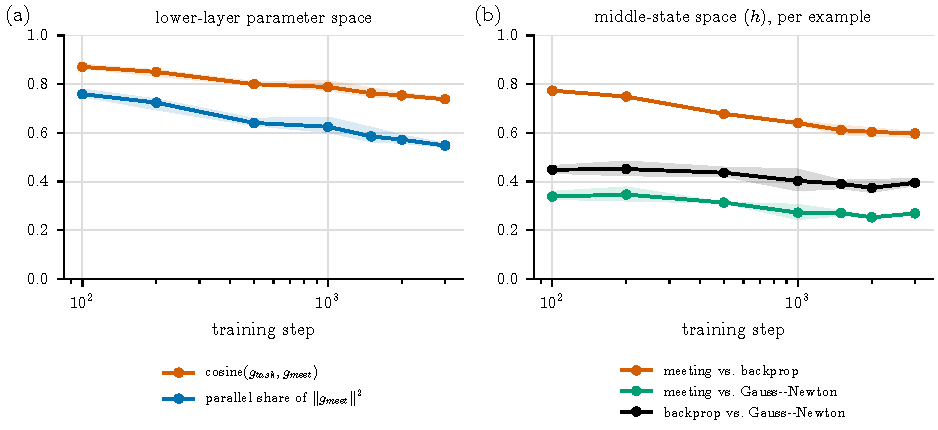
\includegraphics[width=\textwidth]{fig_geometry}
\caption{Geometry of the meeting gradient in arm D (tuned configuration, 3 seeds; lines are means, bands are the range over seeds). (a) In the lower-layer parameter space the meeting gradient is well aligned with the task gradient. (b) In the middle-state space (per example, weighted by the norm of the backpropagation direction) the meeting direction is closer to backpropagation than to the Gauss--Newton direction.}
\label{fig:geometry}
\end{figure}

\begin{caution}
These are first-order, local measurements for one tuned configuration and 3 seeds. A one-step probe that was also run (does a step along the orthogonal part of the meeting gradient lower the loss?) overshoots late in training and should not be quoted as evidence about information in the orthogonal part. The measurements are consistent with the reading that the signal adds little to backpropagation in this network (same direction, small weight); they do not test it.
\end{caution}

\section{Check 2: where does the signal live? Gradient concentration}\label{sec:concentration}
Because the target $b$ equals $h$ when $G(\onehot)=G(p)$, the meeting direction vanishes on examples the network already classifies confidently. The same is true for the task gradient: the gradient of the cross-entropy at the logits is $p-\onehot$, which is tiny for a confident correct prediction. If both signals are concentrated on a few examples, then a method that computes gradients for only those examples loses little. This was measured directly on the baseline (arm A, 3 seeds, 16 fixed batches per checkpoint; plan and rule committed before the run). \Cref{fig:concentration} shows the share of the per-example gradient norm that lies in the top fraction of rows by loss: the top $30\%$ of rows hold $90\%$ of it at step 100, $98.1\%$ at step 500 and $99.7\%$ at step 3\,000, whereas $30\%$ of rows chosen at random hold only $25$--$33\%$. The cosine between the gradient of the top $30\%$ and the full gradient is $0.994$--$1.000$, and the part of the gradient that would be omitted is $10.5\%$ at step 100, $1.6\%$ at step 500 and $0.7\%$ at step 1\,000. The meeting gradient (measured in the run of Check~1) is similarly concentrated: from step 500 on, $97$--$99\%$ of its norm lies in the top $30\%$ of rows by loss, and the correlation between a row's loss and the norm of its meeting direction is $0.99$.

\begin{figure}[t]
\centering
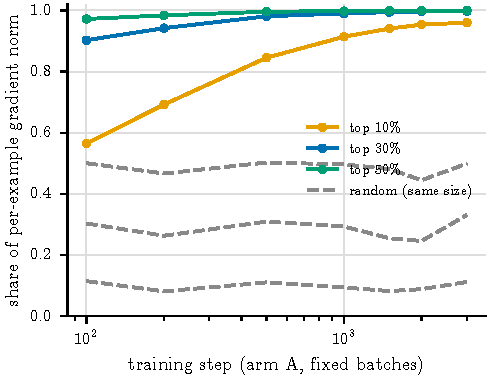
\includegraphics[width=0.62\textwidth]{fig_concentration}
\caption{Share of the per-example gradient norm in the top fraction of rows by loss (solid, three kept fractions) and in an equally sized random subset (dashed), for the baseline trained with the full gradient. The top $30\%$ of rows hold more than $98\%$ of the gradient from step 500 on.}
\label{fig:concentration}
\end{figure}

This is a \emph{necessary condition} for a selective backward pass, measured on a model trained with the full gradient. It does not show that training with a selective pass converges as fast, which is why Study~2 is a test and not a consequence.

\section{Check 3: is it a matter of strength? Dose-response}\label{sec:dose}
A null result invites the reply ``the signal was too weak''. To test this, the meeting term was replaced by a version whose strength is set \emph{relative to the task gradient}. For each example $i$, with $u_i=G(\onehot)-G(p)$ and $n_i=\|\partial\Ltask/\partial h_i\|$,
\begin{equation}
\mathcal{L}_{\rho} = -\rho\, r(t) \sum_i n_i \left\langle \frac{u_i}{\|u_i\|},\, h_i \right\rangle ,
\end{equation}
so that the gradient at $h_i$ has norm $\rho\,r(t)\,n_i$ and points against $u_i$, and $\rho=0$ is the baseline. The learned $G$ is trained as in arm D. The dose $\rho$ was swept at the \emph{baseline's} tuned settings (ReLU, AdamW, cosine schedule, 3\,000 steps), with $10$ paired seeds per block and a ramp of 200 steps: $\rho\in\{0,0.1,0.3,1,3\}$ with ReLU, the low doses $\{0,0.001,0.003,0.01,0.03\}$ with ReLU, and $\{0,0.1,0.3,1,3\}$ with $\tanh$ (whose hyper-parameters were not re-tuned). Each block has its own $\rho=0$ control on the same seeds.

\begin{figure}[t]
\centering
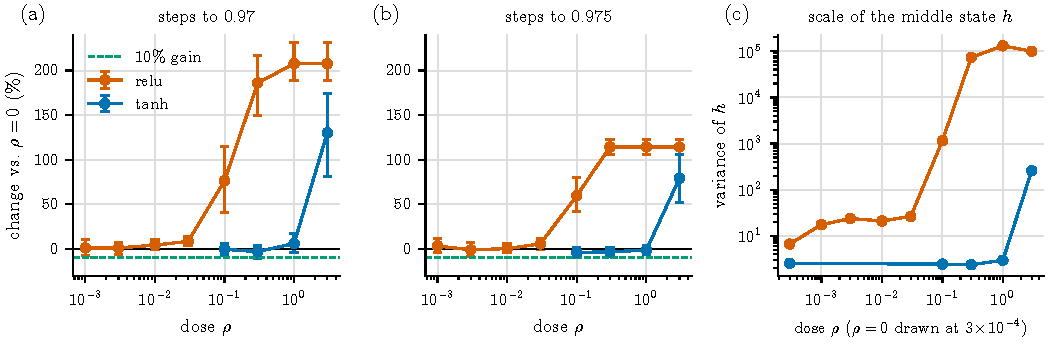
\includegraphics[width=\textwidth]{fig_dose}
\caption{Dose-response of the meeting signal (10 paired seeds per dose; $95\%$ bootstrap intervals). (a), (b) Change in the steps to reach $0.97$ and $0.975$ relative to the same seeds at $\rho=0$; a value above zero is slower. The dashed green line marks a $10\%$ gain. Values of $+208\%$ and $+114\%$ are the ceiling of the metric: every run failed to reach the target and was charged all 3\,000 steps. (c) Median variance of the middle state $h$ after step 1\,000.}
\label{fig:dose}
\end{figure}

\paragraph{Results.} No dose speeds up training (\cref{fig:dose}). With ReLU the harm grows with the dose: $+76\%$ and $+60\%$ more steps to $0.97$ and $0.975$ at $\rho=0.1$, and at $\rho\ge0.3$ almost all runs failed to reach the target within 3\,000 steps. The lowest doses (0.001--0.03) change the steps by $-1\%$ to $+9\%$, with harm appearing at $\rho=0.03$. With $\tanh$ the signal is strongly aligned with the task gradient (cosine about $+0.8$) and the effect is flat up to $\rho=1$ (changes between $-4\%$ and $+6\%$, all intervals contain 0), but at $\rho=3$ training breaks down ($+130\%$ and $+79\%$ steps). In ReLU the variance of the middle state grows from the lowest dose on, from about 7 at $\rho=0$ to $10^3$--$10^5$ at $\rho\ge0.1$, and the inverse loss follows it; the final validation accuracy falls from $0.980$ to $0.976$ at $\rho=0.1$ and to $0.78$--$0.83$ at $\rho\ge1$.

\paragraph{What this shows.} (1) The null result of Study 1 is not a case of ``a too weak signal that more strength would rescue'': more strength made things clearly worse in ReLU and no better in $\tanh$, in no case giving a $10\%$ gain. (2) The signal is not wrong in direction (the alignment in $\tanh$ is $+0.8$), but it adds nothing at these settings, which is what the geometry suggested. (3) A design lesson: a meeting term that is linear in $h$, with strength tied to the task gradient, is unstable when the activation does not saturate; a method that uses such a signal would need a bound or a normalisation of the scale of the middle state. The conjecture that the unbounded scale of $h$ is the cause of the ReLU failure is a hypothesis; a first expectation that $\tanh$ would bound $h$ and so prevent the failure was wrong, because at $\rho=3$ the variance of $h$ also grows in $\tanh$.

\section{What was not tested}\label{sec:notrun}
Three further checks were planned and not run: an \emph{oracle-target} arm that replaces the learned $G$ with the exact Gauss--Newton or a damped logit-space target (to separate ``bad target'' from ``redundant signal''); a \emph{replacement} test (is the meeting signal sufficient to train the lower half with backpropagation cut, which is the use for which target propagation was designed?); and a \emph{deep-network SGD} study (a deeper plain MLP, SGD with momentum, against deep supervision). The project notes plan them as ``checks B, D and C'', and the project records do not contain a decision to drop them; they were simply not run before the work moved on to the selective-backward idea that check 2 suggested. A further line of work (fixes to the quality or cost of $G$) was planned to open only if one of the checks showed a reduction in steps large enough to pay the overhead, which no check did. The additive use of the signal is therefore exhausted by Studies~1 and the three checks, while the question of whether the signal can \emph{replace} part of backpropagation at a lower cost, and whether a better target changes the picture, remains open (\cref{sec:future}).

\section{Interpretation}
The evidence supports, but does not prove, a \emph{redundancy} reading: the meeting signal points in nearly the same direction as backpropagation, lives on the same few high-loss rows, is small at its tuned weight, and gives no benefit at any tested larger weight. If the signal does nothing that backpropagation does not already do, then adding it can only add cost. A stronger reading (that no auxiliary target-propagation signal could help) is not supported: only the learned inverse $G$ of this form, in this network, with AdamW, was tested.
